\documentclass[letterpaper,twoside,12pt]{article}
\usepackage{graphicx}
\usepackage[margin=0.8in]{geometry}


\title{ER2201 Session Delay Closures}
%\author[1]{L. Benkevitch}

\begin{document}

\maketitle

The closure delays are calculated for the baseline triangles when all the three scans are available. The available times for each baseline are shown in Fig.~\ref{time_gaps}.

The distribution plots shown below use different colors for each triangle. The legend for colors used is provided in each Figure. Figs.~\ref{mbd} and~\ref{sbd} show closure delay distributions over 5.5 hours and histograms of magnitudes for the multi-band and single-band delays computed for the residual mbd and sbd. Both show better concentrations near zero for the PolConvert products.

At the time of ER2201 session, the band-D was absent at the station Y (Yj, RAEGYEB, 13-m at Yebes, Spain), so the closure delay calculations of the total multi-band and single-band delays fail for the EVY, EMY, ESY, ETY, MSY, MTY, MVY, SVY, TVY triangles, containing the station Y. However, the delay closures for triangles EMV, ESV, ETV, EMS, EMT, MSV, MTV (without the Y station) demonstrate good behavior. 

To show the difference, Figs.~\ref{mbdYnY} and~\ref{sbdYnY} show the residual mbd and sbd closures for the triangles without the station Y and those with station Y separately. Omitting the triangles with Y results in better closure distributions. 

The total mbd and sbd closures are shown in Figs.~\ref{tot_mbd} and~\ref{tot_sbd}, also without and with station Y, separately. Only closures without the Y station show good distributions.  




\begin{figure}[h!]
  %\begin{center}
  \centering
  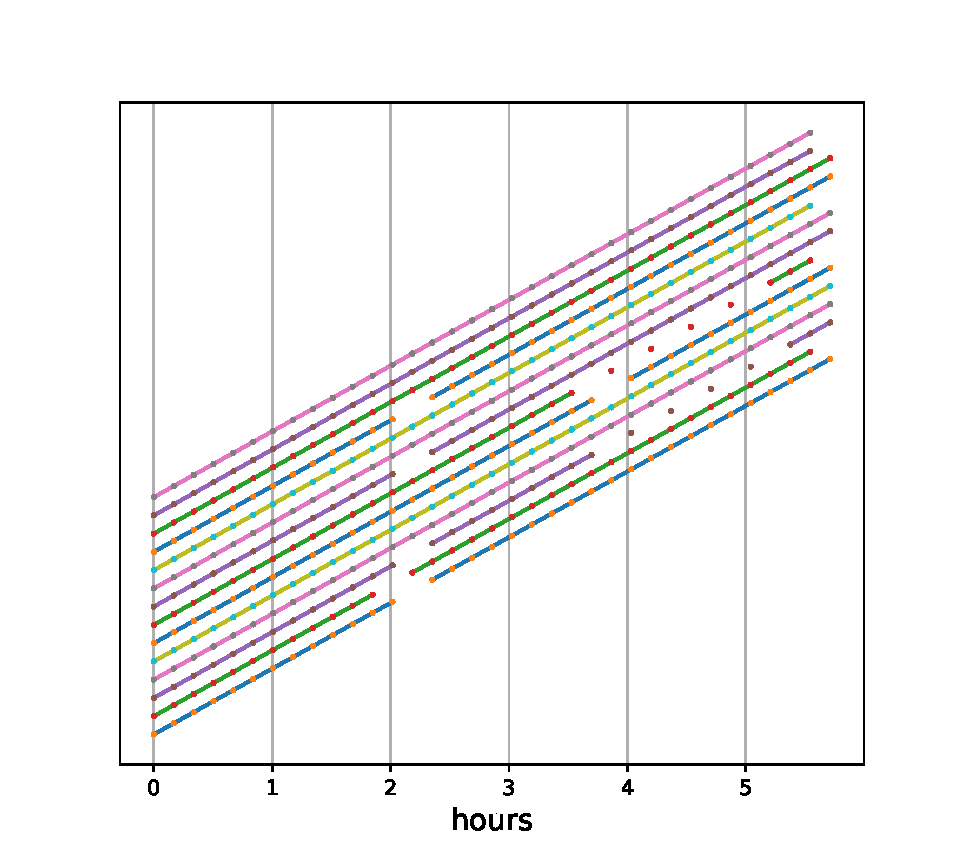
\includegraphics[width=30pc]{Gaps_in_Time.pdf}
  \caption{\small Scan times for all the baselines. The scan times are marked with black dots. The missing scans are shown as white spaces. }
  \label{time_gaps}
  %\end{center}
\end{figure}

\begin{figure}[h!]
  %\begin{center}
  \centering
  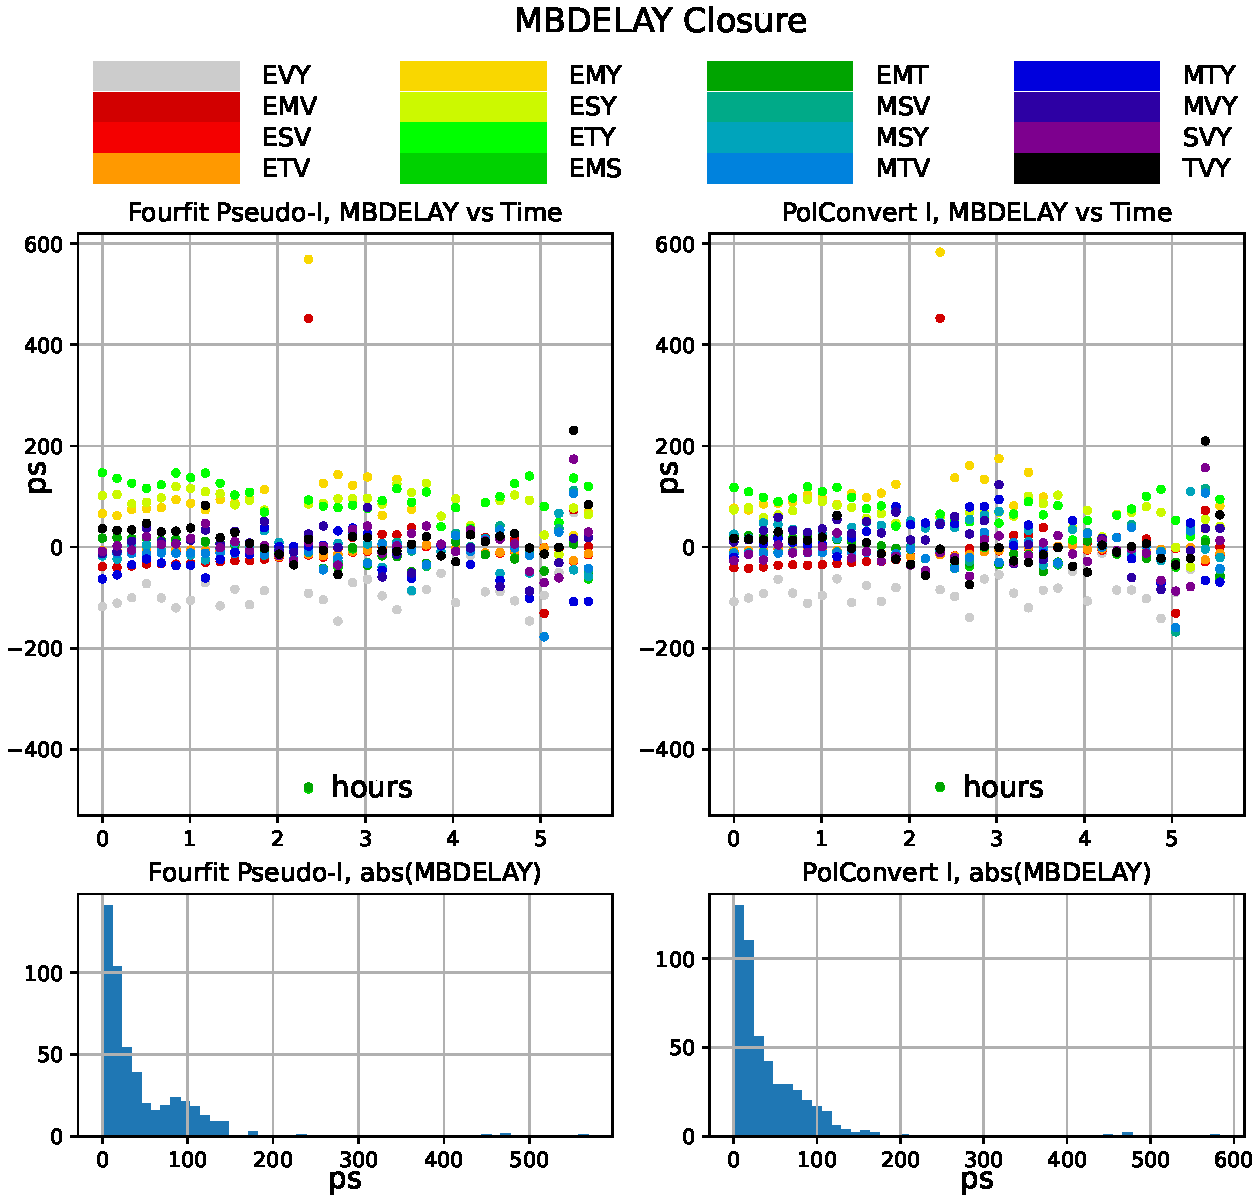
\includegraphics[width=40pc]{MBDELAY_Closure_Delay.pdf}
  \caption{\small MBDELAY closure delay distributions over 5.5 hours and their histograms.}
  \label{mbd}
  %\end{center}
\end{figure}


\begin{figure}[ht!]
  \begin{center}
  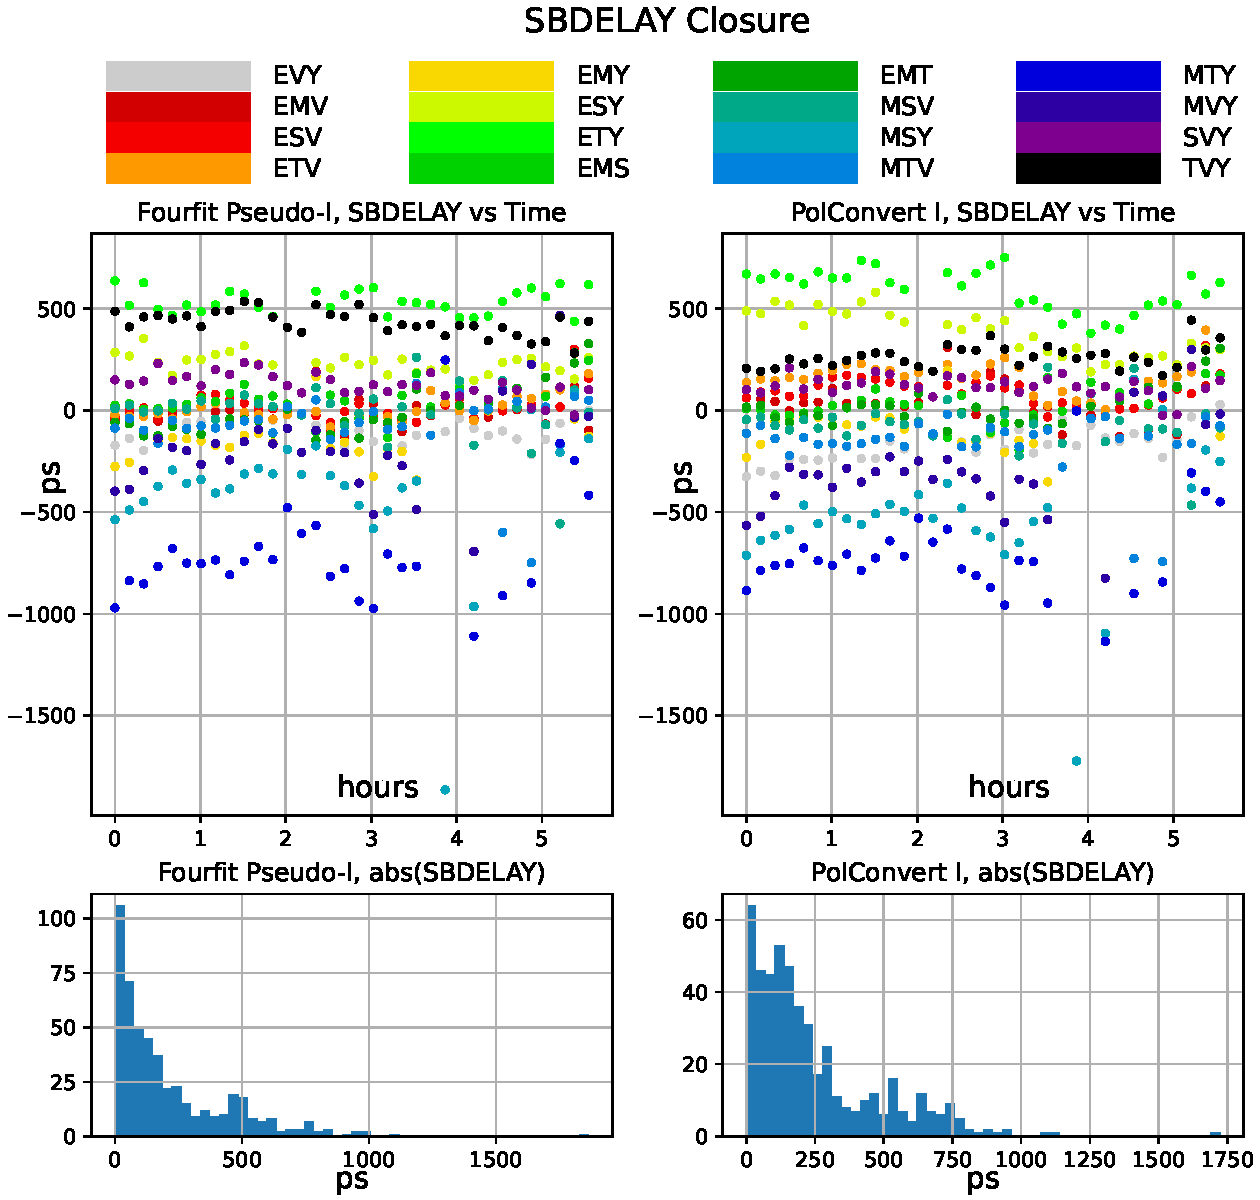
\includegraphics[width=40pc]{SBDELAY_Closure_Delay.pdf}
  \caption{\small SBDELAY closure delay distributions over 5.5 hours and their histograms.}
  \label{sbd}
  \end{center}
\end{figure}


\begin{figure}[h!]
  %\begin{center}
  \centering
  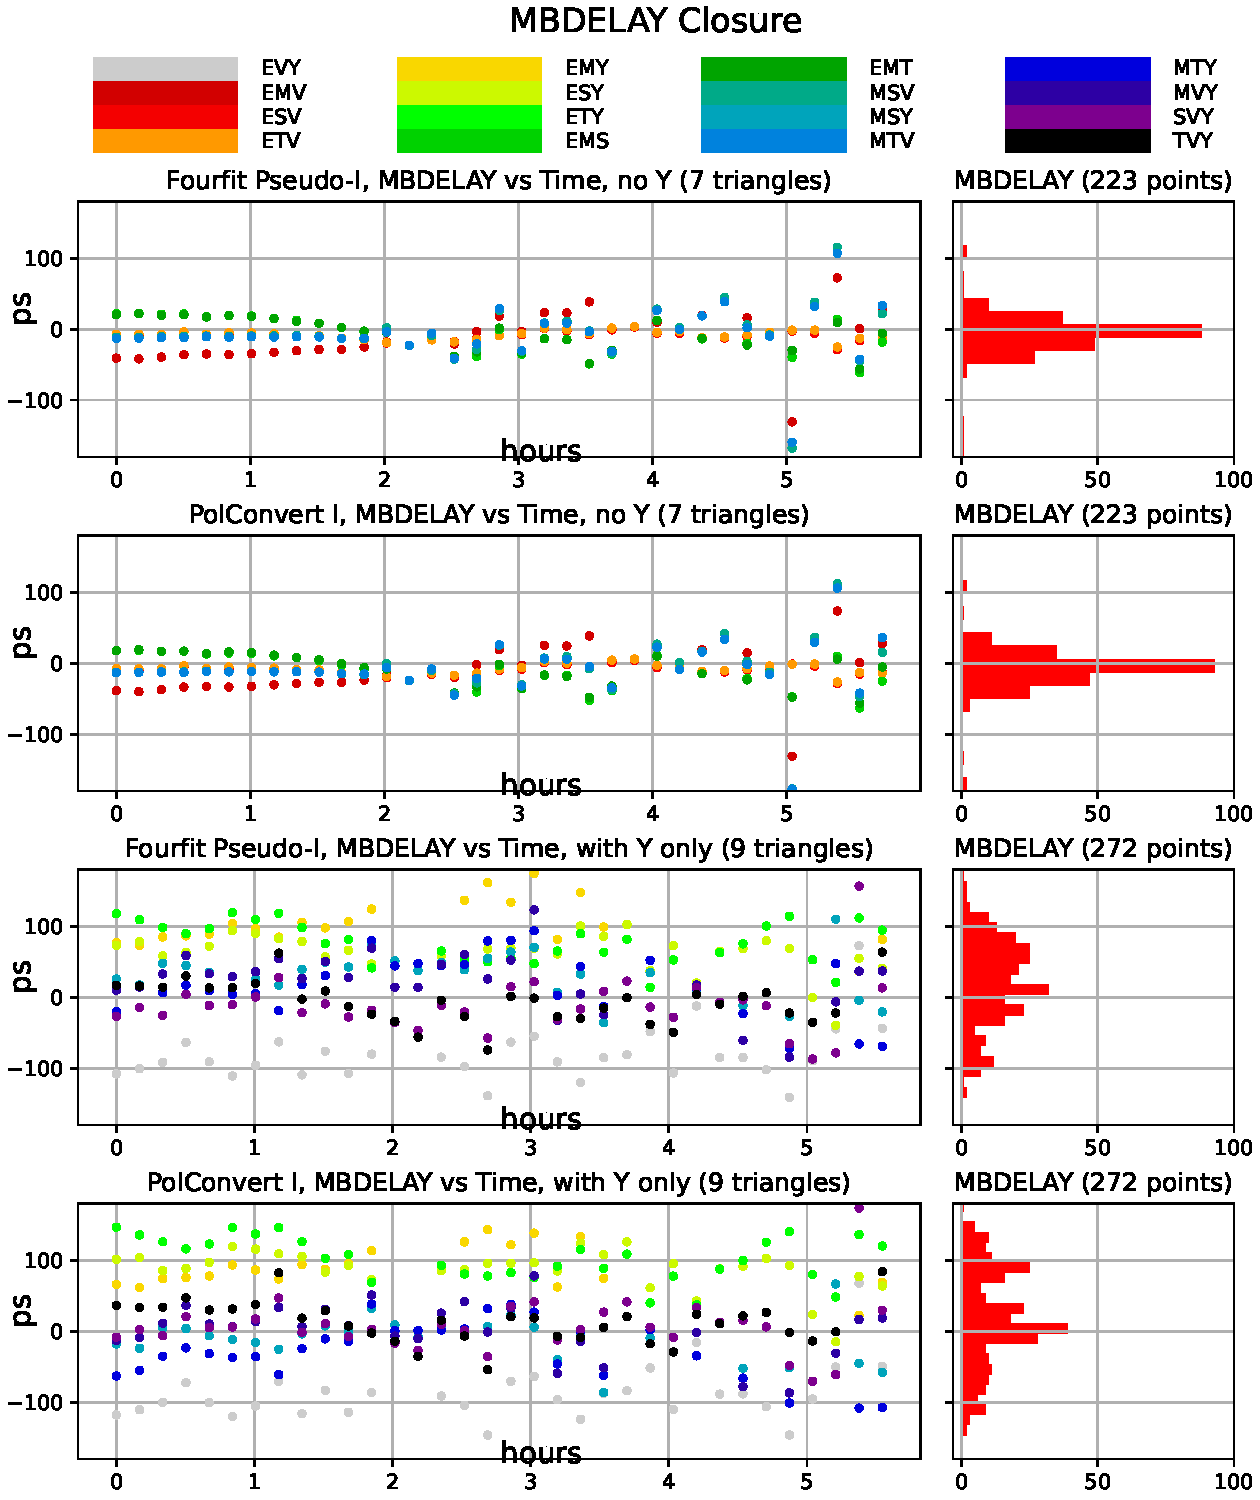
\includegraphics[width=40pc]{MBDELAY_Closure_Delay_Y_no_Y.pdf}
  \caption{\small MBDELAY closure delay distributions over 5.5 hours and their histograms. In the upper and lower panels the results for data without the Y station and with the Y station are shown separately.}
  \label{mbdYnY}
  %\end{center}
\end{figure}


\begin{figure}[ht!]
  \begin{center}
  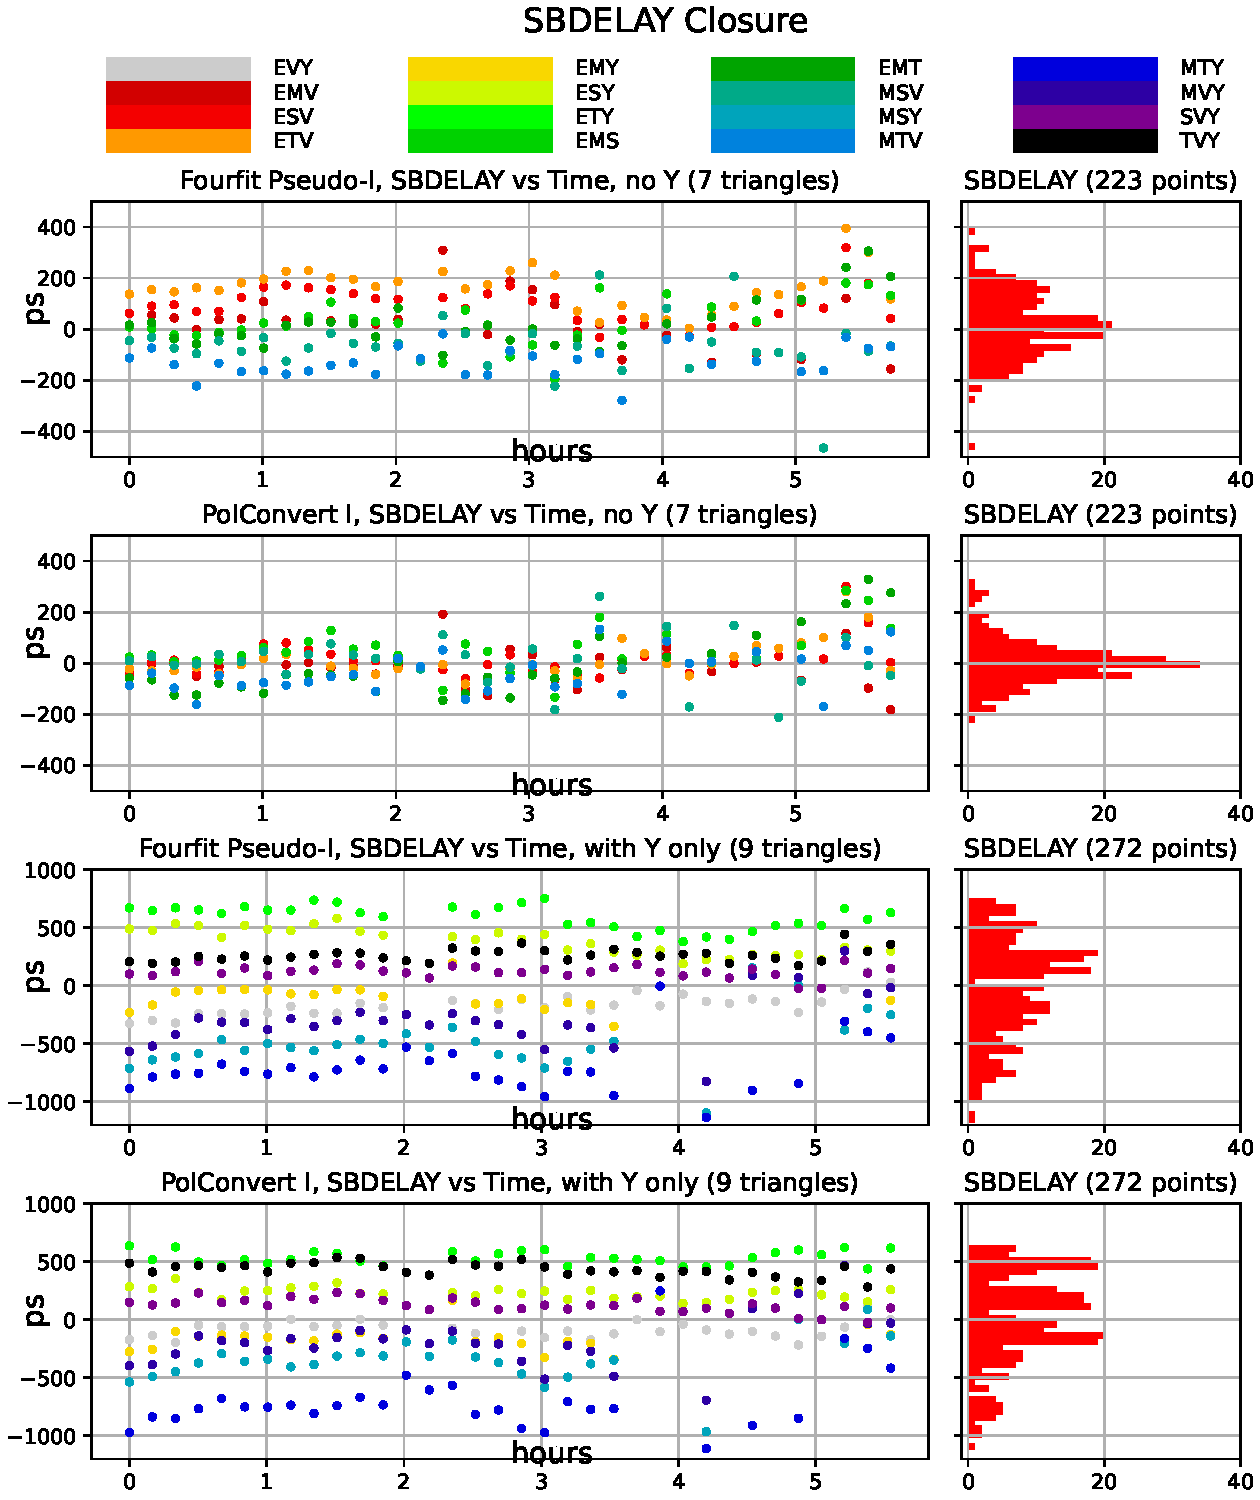
\includegraphics[width=40pc]{SBDELAY_Closure_Delay_Y_no_Y.pdf}
  \caption{\small SBDELAY closure delay distributions over 5.5 hours and their histograms. In the upper and lower panels the results for data without the Y station and with the Y station are shown separately.}
  \label{sbdYnY}
  \end{center}
\end{figure}


\begin{figure}[ht!]
  \begin{center}
  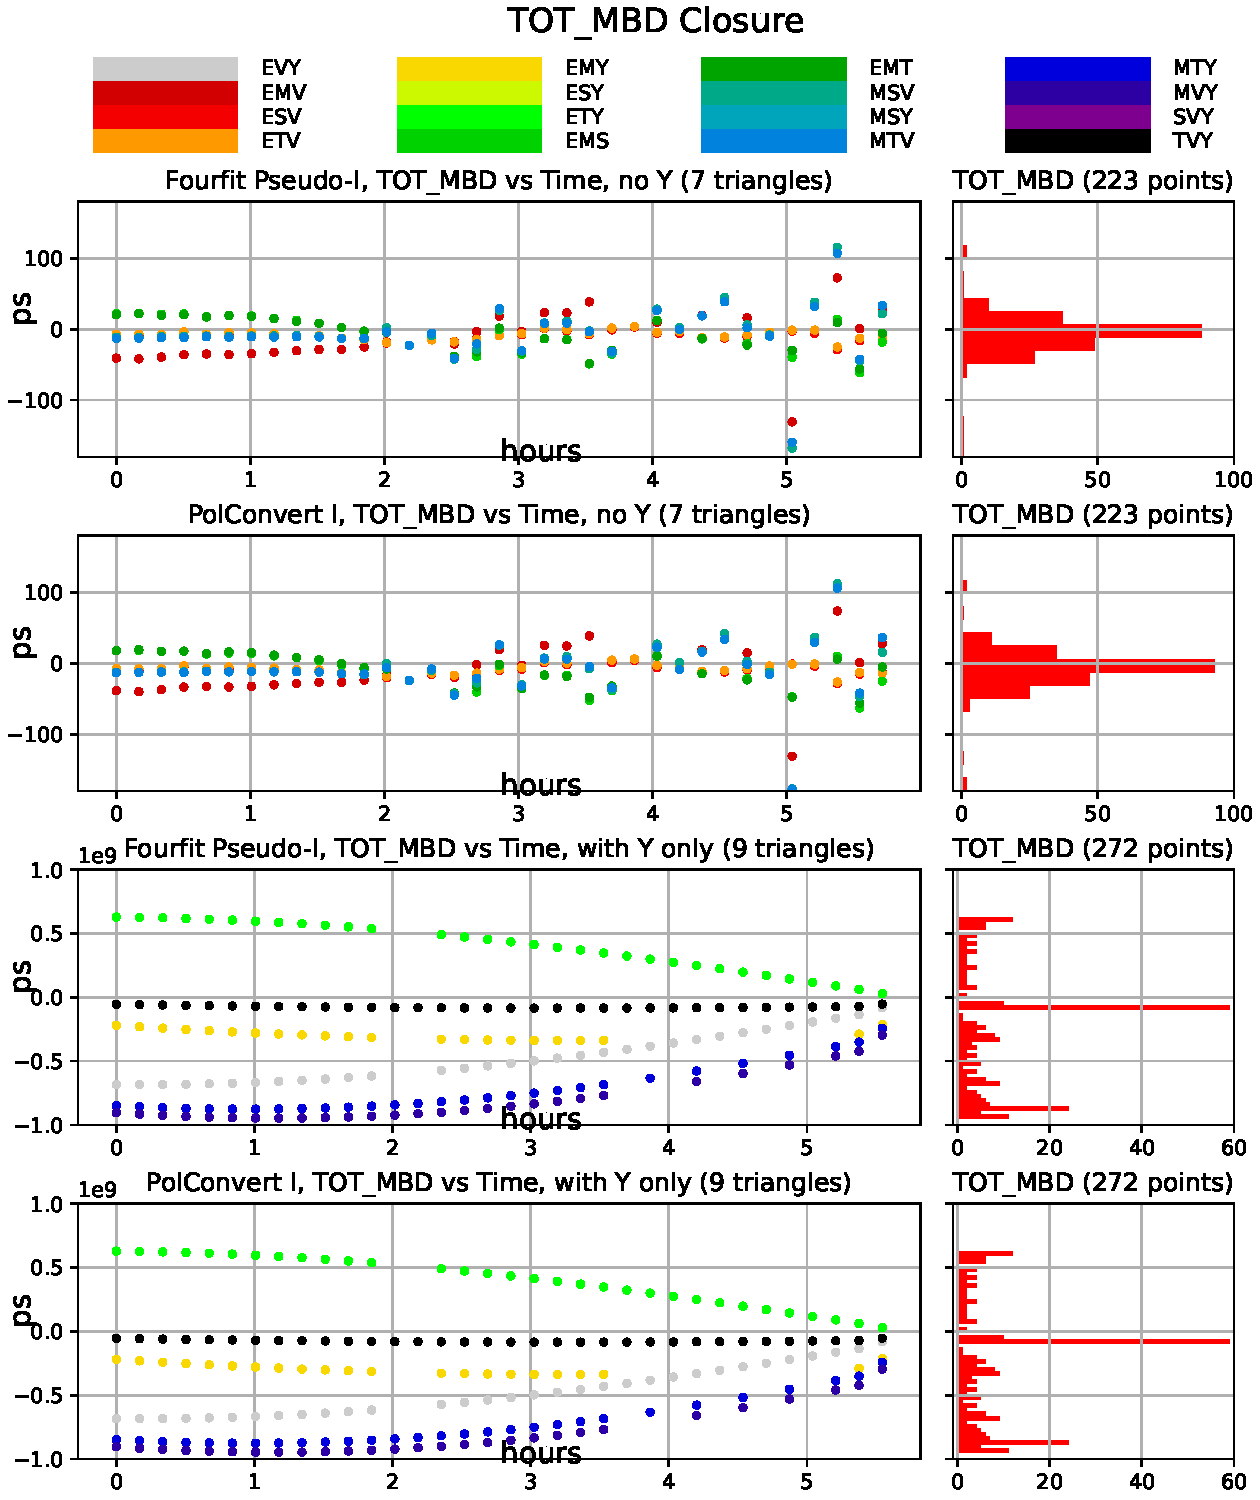
\includegraphics[width=40pc]{TOT_MBD_Closure_Delay_Y_no_Y.pdf}
  \caption{\small Total MBDELAY closure delay distributions over 5.5 hours and their histograms. In the upper and lower panels the results for data without the Y station and with the Y station are shown separately.}
  \label{tot_mbd}
  \end{center}
\end{figure}


\begin{figure}[ht!]
  \begin{center}
  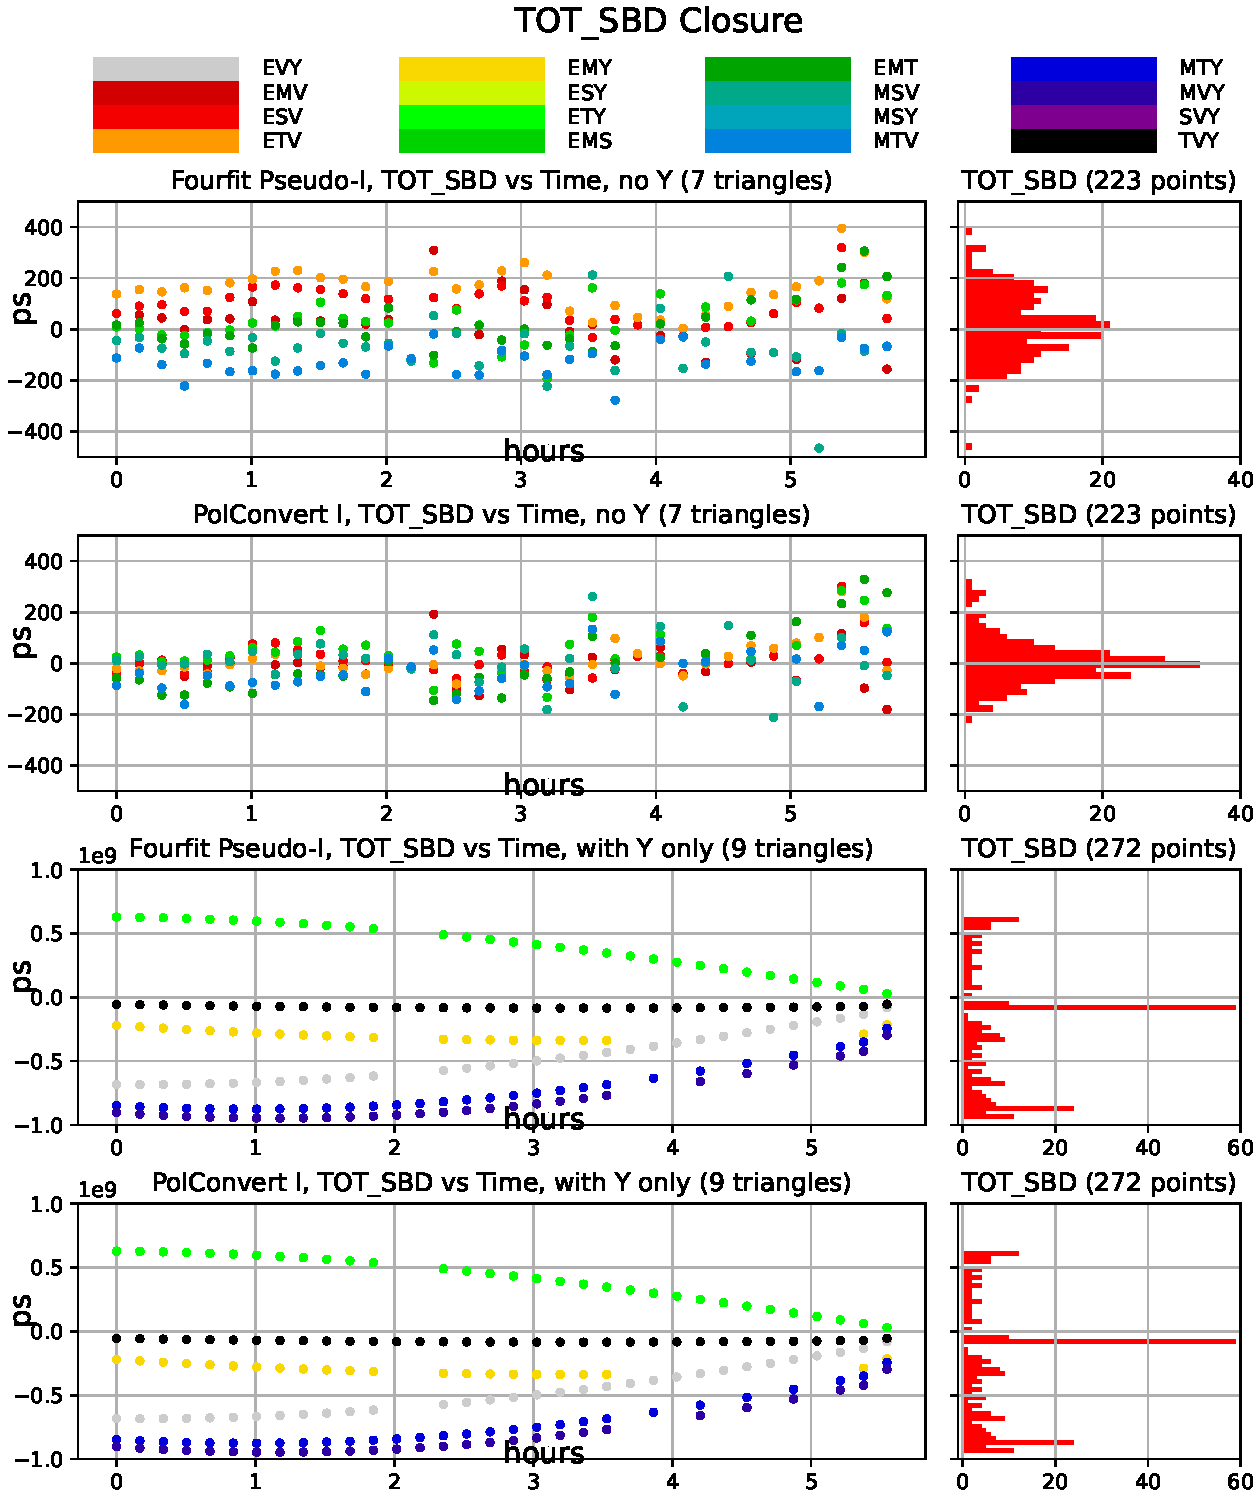
\includegraphics[width=40pc]{TOT_SBD_Closure_Delay_Y_no_Y.pdf}
  \caption{\small Total SBDELAY closure delay distributions over 5.5 hours and their histograms. In the upper and lower panels the results for data without the Y station and with the Y station are shown separately.}
  \label{tot_sbd}
  \end{center}
\end{figure}




\end{document}








